\chapter{Lenna --- \emph{Preprocessing}}

Before trying to detect paragraphs, lines and characters in the image, and then recognizing the characters, we have to "clean" the image. In this chapter we will describe the different algorithm we implemented in this purpose.

\section{Binarization}
This is the first algorithm we wrote, because it was easy, essential and a good
start to learn the library's basic functions. We first implemented the most
naive algorithm you could think of: computing each pixel's luminosity by
averaging its RGB components, and applying a thresholding. Every pixel below 127
was considered white and every pixel above 128 was considered black.
Of course this was not the definitive algorithm.\\

We could have enhanced it by setting the threshold to the average luminosity,
but it wouldn't have been much better. We instead looked for a better algorithm
and found the Otsu's method to be fitting exactly our purposes. Moreover it is
pretty straightforward to implement. Basically Otsu's method is just a way of
finding the ideal threshold. The ideal threshold is defined as being the one
which minimize the variance between the two classes formed by that threshold.
Therefore it has to try every possible threshold and compute every time the
variance of each class. Thanksfully a little mathematical trick allows us to
significantly reduce the time complexity by maximizing the between-class
variance instead of minimizing the within-class variance.\\

\section{Noise reduction}

We tried two method to reduce the noise in the image: gaussian blur and median
filter. We were unsatisfied with both because letters were less readable after
the filter, and they hardly reduced the noise. We will have to search better
method for noise reduction, but for now we will simply use an algorithm that
removes every black pixel surounded by four white pixels. Even if this is a much
simpler algorithm, letter shapes are saved and some noise is removed.

\section{Rotation}

Il est très difficile voir impossible (ou du moins contre-productif) de
détecter des zones de textes, caractères, mots dans une image si cette image
n'est pas droite. C'est pourquoi il est nécessaire, au cours de l'étape de
pré-traitement \emph{pre-processing}, de roter l'image fournie par l'utilisateur
afin qu'elle soit bien adaptée aux étapes de segmentation et d'identification
des caractères. \\

\subsection{Implémentation naive}

Une implémentation naive de la rotation serait l'algorithme suivant. C'est
celui que nous utilisions à la première soutenance mais qui posait quelques
soucis. \\

\begin{itemize}
  \item{Input} \\
    \begin{itemize}
      \item Image de base
      \item Angle de rotation $\theta$
    \end{itemize}
  \item{Output}
    \begin{itemize}
      \item Image rotée
    \end{itemize}
\end{itemize}

\begin{enumerate}

  \item Soit $(w, h)$ les dimensions de l'image de base. Calculer les dimensions
    $(nw, nh)$ de l'image après qu'une rotation d'angle $\theta$ soit appliquée
    sur l'image de base. Visuellement, les dimensions de l'image de base et de
    l'image rotée sont liées par une simple relation trigonométrique.
  \begin{center}
    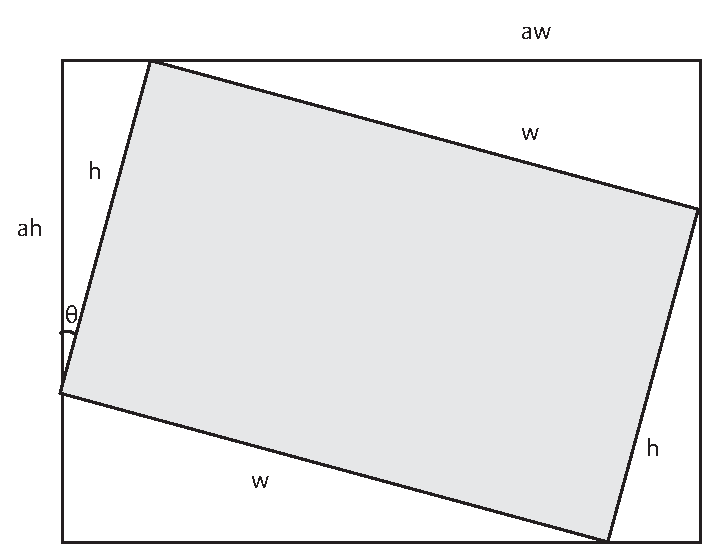
\includegraphics[scale=0.75]{chapters/Pictures/toogy/rotation-new-size.eps}
  \end{center}

  \item Créer une nouvelle image de dimensions $(nw, nh)$ remplie de blanc.

  \item Pour chaque pixel de la nouvelle image, matérialisé par ses coordonnées
    $(x,y)$ dans l'image rotée, calculer ses anciennes coordonnées $(x',y')$
    dans l'image de base. Pour ce faire, on a la relation: \\ 
    $$\begin{pmatrix}x'\\y'\end{pmatrix} =
      \begin{pmatrix}
        \cos\theta & -\sin\theta \\
        \sin\theta & \cos\theta
      \end{pmatrix}
    \begin{pmatrix}
      x \\
      y
    \end{pmatrix}$$

  \item Arrondir ces nouvelles coordonnées et donner aux pixel $(x,y)$ de la
    nouvelle image la couleur du pixel $(x',y')$ de l'image de base. Renvoyer
    l'image.

\end{enumerate}

Cependant, cet algorithme déforme légèrement l'image. Ici, il s'agit de texte et
cette petite déformation réduit énormément sa lisibilité; pour l'homme comme
pour la machine. Il s'agit donc d'être plus intelligent.

\subsection{Interpolation Bilinéaire}

\subsubsection{Interpolation mathématique}

En mathématiques, une interpolation consiste à se servir de données déjà
existante pour approximer des données qui nous manquent. \\

Une interpolation peut se faire de plusieurs façons; plus ou moins précises.
Bien sûr, qui dit plus de précision dit plus de temps de calcul.

\subsubsection{Interpolation bilinéaire appliquée à la rotation}

Ici, il s'agit de se servir des pixels de notre image de base (nos données) pour
déterminer les pixels de notre nouvelle image (les données que nous allons
interpoler). \\

Plusieurs algorithmes d'interpolation existent :
\begin{itemize}
  \item{Nearest-neighbor Interpolation} : le plus simple, il consiste à faire
    la moyenne des composantes $(r,g,b)$ des pixels voisins de notre pixel
    $(x',y')$. C'est le plus rapide.
  \item{Bilinear Interpolation} : un peu plus complexe, il s'agit ici de faire
    deux interpolations linéaires : une entre les deux pixels au dessus de
    $(x',y')$ et une autre entre les deux pixels en dessous de $(x',y')$ (les
    valeurs $x'$ et $y'$ n'étant évidemment pas approximées mais bien située
    entre les entiers de l'arrondi supérieure et de l'arrondi inférieur des
    coordonnées).
    \begin{center}
      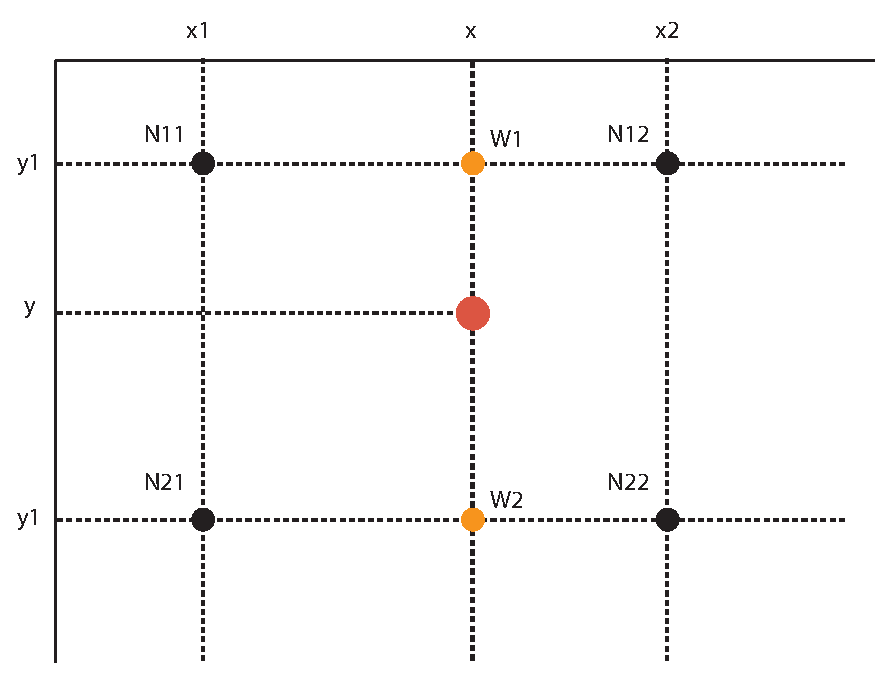
\includegraphics[scale=0.75]{chapters/Pictures/toogy/bilinear.eps}
    \end{center}
    On a alors : \\
    $$W_{1} = \frac{x_{2} - x}{x_{2} - x_{1}} N_{11}
    + \frac{x - x_{1}}{x_{2} - x_{1}} N_{21}$$ \\
    $$\text{et } W_{2} = \frac{x_{2} - x}{x_{2} - x_{1}} N_{12}
    + \frac{x - x_{1}}{x_{2} - x_{1}} N_{22}$$ \\
    Les nouvelles composantes du pixel peuvent alors être calculée via la
    formule \\
    $$R = \frac{y_{2} - y}{y_{2} - y_{1}} W_{1}
    + \frac{y - y_{1}}{y_{2} - y_{1}} W_{2} \text{ \emph{(cas de la
    composante rouge du pixel)}}$$
  \item{Bicubic Interpolation} : plus longue de part son temps de calcul, c'est
    le même principle que pour l'interpolatian bicubique sauf que 8 pixels sont
    étudiés au lieu de 4. Elle donne des résultats plus esthétiques qui ne sont
    pas vraiment utiles dans notre cas.
\end{itemize}

\subsection{Angle detection}

\subsubsection{Hough transform}

The Hough transform is a general method for finding lines and ellipses in an
image. It is often used because once the mathematical principle is understood,
it is not that hard to implement, and it has a much lower time complexity and
better results than some other methods like Fourier transform. For our purposes,
we only need to handle the most simple case: line detection in a binary image.\\

The Hough transform relies on a very particular representation of lines of the
plane: instead of being as the two parameters $a$ and $b$ in the classical
equation $y = ax + b$, it is described as the couple $(r, \theta)$ where $r$ is
the distance of the line from the origin and $\theta$ is the angle of this
distance from the absciss.\\

\begin{center}
\end{center}

How is this representation useful? It comes from the fact that, given a point
of coordinates $(x, y)$ and the angle $\theta$ of a line going through this
point, we can express very simply the distance $r$ of the line from the origin.
The equation is as follows:\\

$r = x\cos\theta + y\sin\theta$\\

So for a point of coordinates $(x, y)$ we can plot the graph of $r$ in function
of $\theta$. It is easy to guess from the equation that it will be a sinusoid.
This sinusoid represents the set of lines going through this particular point.
Now if we store this graph on an accumulator, and add to this accumulator the
sinusoid of every other points, here is what happens:\\

\begin{center}
\end{center}

Clearly there is a point where all sinusoids cross. The coordinates of this
point represents the values $r$ and $\theta$ of the line going through every
point at once.

\subsubsection{More preprocessing}

There is still one thing to fix before applying the Hough transform to our
scanned image: A text doesn't appears as a straight line. We tried to apply the
Hough transform directly to a binarized document, but most of the time it would
find either the diagonal of the document (since the diagonal goes through more
black points than an horizontal or a vertical line), or the angle of a prominent
bookbinding or document border. After a few researches, we came with our own
solution: we first find `blocks' of pixels, defined as being a set of conjoint
pixels. We remove every pixel of this block and replace them by a single pixel
at the center of the block. There are two purposes to this algorithm: replacing
every character by its center to make text lines apparent, and reducing the
importance of large blocks of pixels as bookbindings and images in the Hough
transform. Here is a sample output:\\

\begin{figure}[h!]\
    \centering
    \caption{input image}
\end{figure}
\begin{figure}[h!]\
    \centering
    \caption{center of each block}
\end{figure}
\begin{figure}[h!]\
    \centering
    \caption{line found by the Hough transform}
\end{figure}

This method has a major flaw that we wish to correct before the end of the
project: when the noise isn't reduced enough, every separate pixel in the
`noisy zone' is considered a block and gets a huge role in the Hough transform,
potentially leading the angle detection to fail completely. Every further step
of the OCR relies on a perfectly straight image, and it is therefore very
important that we correct this. \\

\section{TODO}

If Lenna is almost finished, some improvements still remain:

\begin{itemize}

    \item{Rotation}: it is divided in two parts: angle detection, which is done
        and the real rotation. The current algorithm gives very poor results. We
        are going to implement bicubic interpolation which is a standard in many
        image editing programs (including Adobe Photoshop).
    
    \item{Noise reduction improvement}: our noise reduction algorithm is not
        strong enough on some images. Sometimes it fails and Freddy cannot work
        with Lenna's output.

    \item{Hough transform preprocess} The method we use has a major flaw that we wish to correct before the end of
        the project: when the noise isn't reduced enough, every separate pixel
        in the "noisy zone" is considered a block and gets a huge role in the
        Hough transform, potentially leading the angle detection to fail
        completely. Every further step of the OCR relies on a perfectly straight
        image, and it is therefore very important that we correct this.

    \item{Image scaling}: Guy may need an image scaling algorithm to display
        thumbnails of user's image.

\end{itemize}
